%!TEX root=../2022_IEEE_DEB_Vizier.tex
\section{Workflow Provenance Model and Runtime}
\label{sec:vizier-workflows}

In this section, we outline Vizier's workflow and versioning model, how we determine which cells of a workflow need to be re-executed if a cell is changed, and introduce the parallel scheduler of the system.

% multi-tiered, two-dimensional provenance model.
% We first relate the model to both classical workflow provenance and modern computational notebooks, then discuss how Vizier's model incorporates a temporal dimension, and finally discuss state invalidation and re-evaluation.

\newcommand{\notebook}{\mathcal N}
\newcommand{\workflow}{\mathcal W}
\newcommand{\artifact}{a}
\newcommand{\nbcell}{c}
\newcommand{\outputval}{o}
\newcommand{\readset}{\vec r}
\newcommand{\writeset}{\vec w}
\newcommand{\globalscope}{\mathcal G}
\newcommand{\outputdomain}{\mathcal O}
\newcommand{\valuedomain}{\mathcal D}
\newcommand{\undefinedval}{\bot}
\newcommand{\unknownval}{\circledcirc}
\newcommand{\keyset}{\texttt{keys}}
\newcommand{\changeset}{\Delta}
\newcommand{\variabledomain}{\Sigma}
\newcommand{\diff}[2]{\Delta(#1, #2)}
\newcommand{\evalnb}[1]{\llbracket #1 \rrbracket}

\begin{figure}
  \centering
  \begin{minipage}{0.9\textwidth}
  \begin{lstlisting}[style=pynotebook]
data = read_csv("social_data.csv")
show(data)
  \end{lstlisting}

  \begin{lstlisting}[style=pynotebook]
data["latlon"] = geocode(data["address"])
show(data)
  \end{lstlisting}

  \begin{lstlisting}[style=pynotebook]
censusblocks = read_geojson("blocks.json")
show(censusblocks)
  \end{lstlisting}

  \begin{lstlisting}[style=pynotebook]
data = spatial_join(data, censusblocks, ["latlon", "geometry"])
count_per_block = data.groupby("block_id").count()
show(count_per_block)
  \end{lstlisting}
  \end{minipage}\\[-4mm]
  \caption{A simplified example notebook}
  \label{fig:exampleNotebook}
\end{figure}

%%%%%%%%%%%%%%%%%%%%%%%%%%%%%%%%%%%%%%%%%%%%%%%%%%%%%%%%%%%%%%%%%%%%%%%%%%%%
%%%%%%%%%%%%%%%%%%%%%%%%%%%%%%%%%%%%%%%%%%%%%%%%%%%%%%%%%%%%%%%%%%%%%%%%%%%%
\subsection{Workflow Model}
\label{sec:vizier:eval}

A workflow in Vizier is a sequence of workflow steps (cells) that can read and write artifacts. 
Artifacts are versioned at the granularity of cells. 
A cell writing an artifact $\artifact$ causes a new version of $\artifact$ to be created. 
We will discuss the APIs Vizier exposes to the data interaction modalities for accessing artifacts in \Cref{sec:multimodality}. 
The semantics of a Vizier workflow is the serial execution of the cells of the workflow, where the latest version of each artifact is passed as input to the cell that will be executed next. 
Thus, as long as the cells themselves are deterministic, the artifact versions created by the execution of a workflow are uniquely determined by the workflow itself.

%%%%%%%%%%%%%%%%%%%%%%%%%%%%%%%%%%%%%%%%%%%%%%%%%%%%%%%%%%%%%%%%%%%%%%%%%%%%%%%%
\begin{exam}
  \label{ex:introduction}
  \Cref{fig:exampleNotebook} shows a notebook with a simplified data ingestion, cleaning, and analysis task.
  The notebook loads the dataset (cell 1), geocodes listed street addresses (cell 2), loads a collection of census blocks (cell 3), and computes summary statistics for each census block (cell 4).
  We use this  notebook to illustrate a key challenge of traditional  notebook architectures.
  %
  The user modifies cell 2 to switch to a different geocoder, potentially requiring re-evaluation of the notebook.
  In this specific notebook, the user had the foresight to write in an idempotent style, making it unnecessary to re-run cell 1 to recover the state needed to run cell 2 correctly.
  It is also unnecessary to re-run cell 3, as it does not depend on the output of cell 2.
  However, in traditional notebooks like Jupyter the burden of deciding which cells to re-evaluate rests on the user, creating added overhead and increasing the chance of errors.
\end{exam}
%%%%%%%%%%%%%%%%%%%%%%%%%%%%%%%%%%%%%%%%%%%%%%%%%%%%%%%%%%%%%%%%%%%%%%%%%%%%%%%%

Formally, a Vizier workflow is a sequence $\notebook = \{ \nbcell_1, \ldots, \nbcell_N \}$ of cells. 
The versions of artifacts valid after execution of cell $\nbcell_i$ are modeled as a global scope $\globalscope$ that maps artifact names to artifact versions or the distinguished symbol $\undefinedval$, which indicates that no version of the artifact has been produced yet.  
A cell $\nbcell$ is a function that takes a scope $\globalscope$ as input and produces an updated scope $\globalscope'$: $\nbcell (\globalscope) = \globalscope'$. 
We use $\readset_{\globalscope,i}$ to denote the names of artifacts accessed by cell $\nbcell_i$ applied to $\globalscope_i$. 
The scope parameter is necessary, because a cell may dynamically decide which artifacts to read based on the content of other artifacts.
%
The result $\evalnb{\notebook}$ of  evaluating workflow $\notebook = \{ \nbcell_1, \ldots, \nbcell_N \}$ is defined as the scope $\globalscope_n$ produced by starting with an empty scope $\globalscope_0$ (where all artifact names are mapped to $\undefinedval$), and by computing $\globalscope_{i} = \nbcell_{i}(\globalscope_{i-1})$.








% Cell evaluation in Vizier happens in notebook-order.

% Each cell is (conceptually) evaluated on the scope emitted by the preceding cell.
% Like the workflow systems that inspired it, Vizier retains inter-cell snapshots of scope to preserve notebook-order evaluation semantics while still allowing users to backtrack.


% Denote by $\globalscope$ a global scope that we will formalize shortly;

% We model a cell $\nbcell (\globalscope) = (\globalscope', \readset, \outputval)$ as a deterministic function applied to a global scope that returns a new global scope $\globalscope'$, a read set $\readset$, and an opaque output object $\outputval$ in $\outputdomain$.
% Evaluating the notebook $\evalnb{\notebook} = (\globalscope_N, [\outputval_1, \ldots, \outputval_N)$ produces a final scope $\globalscope_N$ and a sequence of outputs $\outputval_1, \ldots, \outputval_N$ through straightforward composition, starting with an empty scope $\globalscope_0$.
% %  formalized as:
% % $$(\globalscope_i, \readset_i, \outputval_i) = \nbcell_i(\globalscope_{i-1})$$
% % In the above,

%%%%%%%%%%%%%%%%%%%%%%%%%%%%%%%%%%%%%%%%
\begin{wrapfigure}[8]{r}[0pt]{11cm}
  \centering
  \vspace{-4mm}
  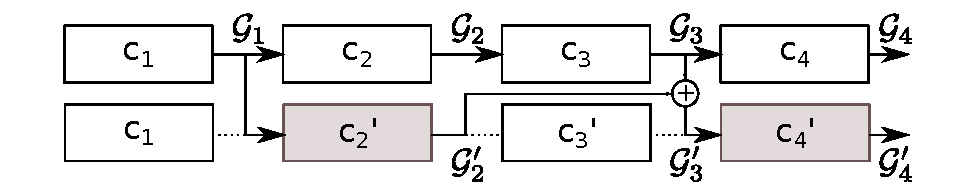
\includegraphics[width=10.5cm]{graphics/eval.pdf}\\[-5mm]
  \caption{Evaluation logic for the example notebook in \Cref{fig:exampleNotebook}.  Edges are labeled with global scope versions.  Cells that are (re-)evaluated are highlighted, dotted lines represent simulated state flow.}
  \label{fig:exampleEval}
\end{wrapfigure}
%%%%%%%%%%%%%%%%%%%%%%%%%%%%%%%%%%%%%%%%
If workflow $\notebook$ is modified by replacing a cell $\nbcell_i$ with a cell $\nbcell_i'$ (denoted as $\notebook[\nbcell_i \backslash \nbcell_i']$), we need to obtain the updated scope $\evalnb{\notebook[\nbcell_i \backslash \nbcell_i']}$. Of course this can be achieved by evaluating $\notebook[\nbcell_i \backslash \nbcell_i']$.
% In lieu of naively re-evaluating the notebook from scratch,
However, to improve performance,  Vizier attempts to update the output of $\evalnb{\notebook}$ by only re-evaluating a subset of the cells.
First, observe that $\globalscope_1, \ldots, \globalscope_{i-1}$ are independent of $\nbcell_i$; and remain unchanged if $\nbcell_i$ is modified.
It is still necessary to have $\globalscope_{i-1}$ to evaluate $\nbcell_i'$; so Vizier caches all intermediate global scopes after evaluating each workflow revision.

% \begin{figure}
%   \centering
%   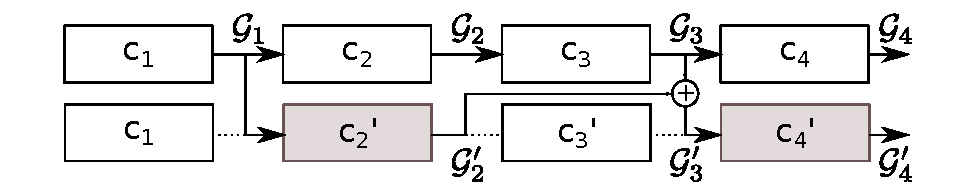
\includegraphics[width=0.7\textwidth]{graphics/eval.pdf}
%   \caption{Evaluation logic for the example notebook in \Cref{fig:exampleNotebook}.  Edges are labeled with global scope versions.  Cells that are (re-)evaluated are highlighted, dotted lines represent simulated state flow.}
%   \label{fig:exampleEval}
% \end{figure}

Naively, we have to still re-evaluate $\nbcell_{i+1}, \ldots, \nbcell_{N}$ using the new scope produced by $\nbcell_i'$. Let us denote the scopes produced by this evaluation as
$\globalscope_{i+1}', \ldots, \globalscope_{n}$.
% $\outputval_{i+1}', \ldots, \outputval_{N}'$.
Vizier uses the readsets $\readset_{\globalscope, i+1}, \ldots, \readset_{\globalscope, N}$, to identify cells $\nbcell_{j}$ for which the same output (artifact versions written by the cell) in $\evalnb{\notebook[\nbcell_i \backslash \nbcell_i']}$ is guaranteed. 
Denote by $\changeset(\globalscope, \globalscope') = \{ k |  \globalscope(k) \neq \globalscope'(k)\}$ the names of artifacts that differ between $\globalscope$ and $\globalscope'$. 
We have to re-execute cell $\nbcell_{i+1}$ if an artifact read by $\nbcell_{i+1}$ has changed, which is the case if $\changeset(\globalscope_i, \globalscope_i') \cap \readset_{\globalscope,i+1} \neq \emptyset$. If $\nbcell_{i+1}$ needs to be re-executed, then we set $\globalscope_{i+1}' = \nbcell_{i+1}(\globalscope_{i}')$. Otherwise, we generate $\globalscope_{i+1}$ by merging the changes made by $\nbcell_{i+1}$ in $\notebook$ to $\globalscope_{i}$ into $\globalscope_{i}'$. That is, for all artifacts $k$ we set
$\globalscope_{i+1}'(k) =   \globalscope_{i+1}(k)$ if $k \in \changeset(\globalscope_i, \globalscope_{i+1})$
and $\globalscope_{i+1}'(k) = \globalscope_{i}'(k)$ otherwise.
% begin{cases}
%   \globalscope_{i+1}(k) &\;\;\;\text{\textbf{if}}\,k \in \changeset(\globalscope_i, \globalscope_{i+1})\\
%   \globalscope_{i}'(k) &\;\;\;\text{\textbf{otherwise}}\\
% \end{cases}$$
 The same approach is applied to decide whether to evaluate or skip the remaining cells in $\notebook[\nbcell_i \backslash {\nbcell_i}']$.


% We formalize a global scope $\globalscope = \{ k_1 \rightarrow v_1, k_2 \rightarrow v_2, \ldots \}$ as a total mapping from an infinite alphabet of variable names $k \in \variabledomain$ to a set of domain values $v \in \valuedomain \cup \{\undefinedval\}$.
% The distinguished symbol $\undefinedval$ denotes an ``undefined'' value, and we assume that finitely many elements of $\variabledomain$ are mapped to non-$\undefinedval$ values (i.e., that $\globalscope$ has finite support).
% Denote by $\keyset(\globalscope) = \{ k | (k \rightarrow v) \in \writeset \wedge v \neq \undefinedval\}$ the keys of the finite support of $\globalscope$.
% Denote by $\changeset(\globalscope, \globalscope') = \{ k |  \globalscope(k) \neq \globalscope'\}$ the change set between $\globalscope$ and $\globalscope'$.

% Given the newly computed $\globalscope_i'$, we want to know if $\nbcell_{i+1}$ needs to be evaluated as well;
% If $\nbcell_{i+1}(\globalscope_i') = (\globalscope_{i+1}', \readset_{i+1}', \outputval_{i+1}')$, we can avoid re-evaluating $\nbcell_{i+1}$ if we can prove that $\outputval_{i+1} = \outputval_{i+1}'$.
% Under the assumption that $\nbcell_{i+1}$ is deterministic with respect to inputs $\readset_{i+1}$, we can guarantee that $\outputval_{i+1} = \outputval_{i+1}'$ when $\readset_{i+1} \cap \changeset(\globalscope_{i}, \globalscope_{i}')$ is empty.
% If we do not need to re-evaluate $\nbcell_{i+1}$, we can reconstruct its output by considering how the original evaluation affected the scope: the write set $\writeset_{i+1} = \changeset(\globalscope_{i}, \globalscope_{i+1})$.
% Concretely $\outputval_{i+1}' = \outputval_{i+1}$, $\readset_{i+1}' = \readset_{i+1}$ and
% $$\globalscope_{i+1}'(k) = \begin{cases}
% \globalscope_{i+1}(k) \textbf{ if } k \in \writeset_{i+1}\\
% \globalscope_{i}'(k) \textbf{ otherwise}
% \end{cases}$$
% \noindent The remaining cells of the notebook are processed in a like manner.

 %%%%%%%%%%%%%%%%%%%%%%%%%%%%%%%%%%%%%%%%%%%%%%%%%%%%%%%%%%%%%%%%%%%%%%%%%%%%%%%%
\begin{exam}
  \Cref{fig:exampleEval} continues the running example from \Cref{ex:introduction}.
  The user has replaced the initial version of cell $\nbcell_2$ with an updated version ${\nbcell_2}'$.
  The global scope produced by preceding cells ($\globalscope_1$) may be re-used unchanged to evaluate ${\nbcell_2}'$, producing scope $\globalscope_2'$.
  $\changeset(\globalscope_2, \globalscope_2')$ is the \lstinline{data} artifact, but the readset of $\nbcell_3$ is empty, and so this cell does not need to be re-evaluated.
  Instead $\globalscope_3'$ is derived by merging variables the cell previously changed (i.e., $\changeset(\globalscope_2, \globalscope_3)$) into the current global scope.
  Finally, Vizier identifies that an element of $\readset_{\globalscope,4}$ (the \lstinline{data} variable) has changed between $\globalscope_3$ and $\globalscope_3'$, necessitating a re-evaluation of cell 4.
\end{exam}
 %%%%%%%%%%%%%%%%%%%%%%%%%%%%%%%%%%%%%%%%%%%%%%%%%%%%%%%%%%%%%%%%%%%%%%%%%%%%%%%%

% \mypara{Frozen Cells}
% Vizier allows users to ``freeze'' cells, temporarily replacing them with no-op commands, but preserving all user-interface elements (including cell outputs), and allowing the cell to be easily re-inserted into the notebook.
% This allows users to quickly disable cells with transient purposes (e.g., sampling cells), or avoid triggering expensive computations while working on an earlier part of the notebook.

% \begin{figure}
%   \centering
%   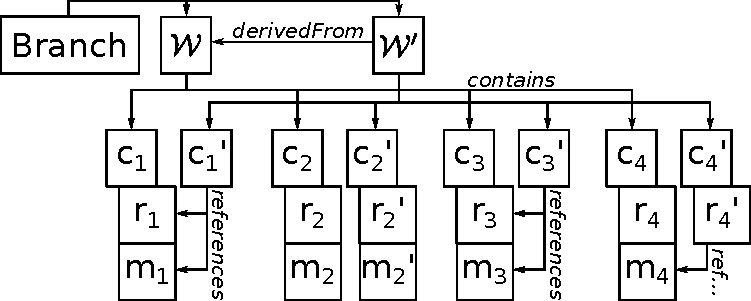
\includegraphics[width=0.45\textwidth]{graphics/history.pdf}\\[-3mm]
%   \caption{History for the running example, assuming cell B was changed as in \Cref{fig:exampleEval}.}
%   \label{fig:exampleHistory}
% \end{figure}

%%%%%%%%%%%%%%%%%%%%%%%%%%%%%%%%%%%%%%%%%%%%%%%%%%%%%%%%%%%%%%%%%%%%%%%%%%%%
%%%%%%%%%%%%%%%%%%%%%%%%%%%%%%%%%%%%%%%%%%%%%%%%%%%%%%%%%%%%%%%%%%%%%%%%%%%%
\subsection{Versioning Workflows}
\label{sec:vizier-history}

%%%%%%%%%%%%%%%%%%%%%%%%%%%%%%%%%%%%%%%%
\begin{wrapfigure}[10]{r}[0pt]{8cm}
  \centering
  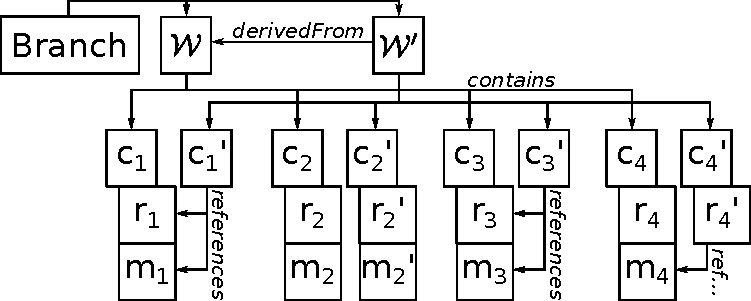
\includegraphics[width=0.45\textwidth]{graphics/history.pdf}\\[-3mm]
  \caption{History for the running example, assuming cell 2 was changed as in \Cref{fig:exampleEval}.}
  \label{fig:exampleHistory}
\end{wrapfigure}
%%%%%%%%%%%%%%%%%%%%%%%%%%%%%%%%%%%%%%%%
Vizier maintains a branching history of the evolution of the notebook.
% We use the term workflow ($\workflow = c_1, \ldots, c_N$) to denote a single state of the notebook.
A cell is further subdivided into (i) \textbf{cell metadata} ($c_i$) that is unique to the workflow (e.g., timestamps and execution status), (ii) \textbf{results} ($r_i$) of executing the cell, and (iii) a \textbf{module} ($m_i$) describing the command executed in the cell.
The latter two components (results and modules) may be shared across workflows.
% In other words, a single cell object acts as a many-to-many-to-many (i.e., 3-ary) relationship between workflow, module, and result entities.
A module object describes the command to be evaluated in a cell.  
This includes its type (e.g., Python or Scala script; SQL query; or one of the graphical widgets), as well as any parameters to the command (e.g., the script itself, or the artifact name to materialize query results as). 
A results object stores references to versions of artifacts in the artifact store created by the execution of the cell. 
We do not materialize the full global scope after each cell, but rather only the changes made to the global scope by the cell (i.e., the cell's write set). 
Any global scope $\globalscope_i$ can be reconstructed from the preceding write sets.

% A results object consists of three items: (i) Messages output by the cell (i.e., $\outputval$), (ii) The cell's readset as a list of name/artifact pairs, and (iii) The cell's writeset as a list of name/artifact pairs.
% Deletion is encoded by writing the distinguished value \texttt{null} to a name.
% As a performance optimization, name/artifact pairs do not embed the artifact literal, but rather a unique artifact identifier.
% This allows for efficient equivalence testing, while avoiding duplication; For example, a ``copy artifact" instruction only needs to clone the artifact identifier under a new name, and not the entire artifact.

% \mypara{Global scope}
% Note that the organizational structure used to persist history information differs from the global scope model used to reason about cell re-use.
% However, the two representations are equivalent.
% Denote by $m_1 \circ m_2$ the right-preferenced composition of \emph{partial} maps $m_1$ and $m_2$ as follows:
% $$m_1 \circ m_2 = \{ k\rightarrow v | (k \rightarrow v) \in m_1 \wedge \not\exists v' \text{ s.t. } (k \rightarrow v') \in m_2 \} \cup m_2$$
% Any global scope $\globalscope_N$ can be recovered by composing the preceding writesets: $\globalscope_N = \globalscope_0 \circ \writeset_1 \circ \ldots \circ \writeset_N$


\begin{exam}
 \Cref{fig:exampleHistory} continues our running example, which in our new terminology is a single branch comprised of two workflows $\workflow_1$ and $\workflow_2$.
  Both notebooks are comprised of four cell objects each.
  Cells 1, 3, and 4 were unchanged between workflows, and so the corresponding cell objects for $\workflow_2$ reference the same module description object as the corresponding cell for $\workflow_1$, while the module descriptions referenced by $\nbcell_2$ and ${\nbcell_2}'$ differ.
  Cells 1 and 3 do not need to be re-evaluated, and so can share their result objects, while Cells 2 and 4 both require re-evaluation and create new result objects.
\end{exam}

%%%%%%%%%%%%%%%%%%%%%%%%%%%%%%%%%%%%%%%%%%%%%%%%%%%%%%%%%%%%%%%%%%%%%%%%%%%%%%%%
\mypara{Workflow and Branch History}
Similar to version control systems like git, each workflow version in Vizier stores a reference to the workflow version it was derived from.
% The difference between workflow versions can be computed by comparing the sequence of modules referenced by the workflow's cells; but simple summary information including the type of change (insert, delete, update) and the affected module (if appropriate) is cached with the workflow object.
A branch is an append-only sequence of workflow versions. % with associated metadata (e.g., a branch name).
The branch contains a reference to the most recent workflow version in the branch. % prior versions are tracked through the series of derived-from references in the workflows themselves.
A new branch may be created from any existing workflow version, including a historical one.

%%%%%%%%%%%%%%%%%%%%%%%%%%%%%%%%%%%%%%%%%%%%%%%%%%%%%%%%%%%%%%%%%%%%%%%%%%%%
%%%%%%%%%%%%%%%%%%%%%%%%%%%%%%%%%%%%%%%%%%%%%%%%%%%%%%%%%%%%%%%%%%%%%%%%%%%%
\subsection{Parallel Scheduler}\label{sec:vizier-scheduler}

The evaluation model presented in \Cref{sec:vizier:eval} relies exclusively on \textit{dynamic provenance}, where Vizier is informed about the readset and writeset of a cell at runtime when the cell accesses artifacts through Vizier's API.
% that assist in determining whether a cell needs to be re-evaluated.
However, dynamic provenance is not always sufficient.
For example, Vizier evaluates cells in parallel where possible, but dynamic provenance is not available until the cell has already been evaluated.
Static provenance, which can derive a cell's read and write sets through static dataflow analysis of its source code, can be computed upfront.
However, static dataflow analysis is of necessity an approximation for some cell types; language features like control flow and dynamic code evaluation can lead to over- (or under-) estimates of the cell's read and write sets. % , especially with respect to a specific global scope.
Vizier uses a novel approach which refines static provenance at runtime using dynamic provenance~\cite{DG22}.

Fundamentally, Vizier's scheduler needs to assign each cell in a running workflow to one of four lifecycle stages: (i) \textbf{DONE} when the cell has a valid result object, (ii) \textbf{PENDING} when the cell depends (directly or transitively) on a cell that does not have a result object, and (iii) \textbf{RUNNING} when the cell's dependencies have a valid result object but the cell itself does not.
We further distinguish as (iv) \textbf{STALE} those cells in the \textbf{PENDING} stage for which we can conclusively determine that re-evaluation is required.
% Lifecycle stage transitions are monotonic.

To manage lifecycle transitions, Vizier's scheduler relies on a combination of static and dynamic provenance~\cite{DG22}.
It uses static provenance to generate an over-approximation on the read and write dependencies of a cell\footnote{As we argue in~\cite{DG22}, to deal with languages that support dynamic code evaluation such as Python, it would be necessary to allow under-approximations of read and write sets (missed data dependencies) and compensate for them at runtime. However, this not implemented in Vizier yet; attempts to dynamically read variables not in the maximal readset are flagged as errors.}.
  % Vizier does not presently support purely dynamic dependencies through e.g., dynamic code evaluation.  A read or write access on a variable not discovered through static analysis triggers an execution error.}.
Accordingly, the scheduler tracks an over-approximation of the read and writesets at each step of the workflow, and refines them when the execution of cell finishes and we know its precise read and write set. 
This approximation is used by Vizier's scheduler to omit cells from re-execution or schedule them for parallel execution if we can determine that it is safe to do so based on these over-approximations.

% Approximate global scopes generalize our prior definition of a global scope by extending the value domain to include the value $\unknownval$, denoting an unresolved value (i.e. variables in an approximate global scope are drawn from $\valuedomain \cup \{\undefinedval, \unknownval\}$).
% Like a regular global scope, an approximate global scope is derived by concatenating writesets ($\globalscope_i = \globalscope_{i-1} \circ \writeset_i$).
% However, if the cell is in a lifecycle stage other than \textbf{DONE}, its previous writeset is not valid.
% Instead, Vizier uses static analysis to derive an upper bound on the writeset $\writeset_{\max} \subseteq \variabledomain$, the maximal set of variables that the cell is allowed to write to.
% When the cell's writeset is not (or may not be) valid, the approximate global scope is instead updated by making each element of $\writeset_{\max}$ an unknown:
% $\globalscope_{i} = \globalscope_{i-1} \circ \{ k \rightarrow \unknownval | k \in \writeset_{\max, i} \}$

% \Cref{alg:lifecycleStage} explains how Vizier derives the lifecycle stage of a cell from the global scope emitted by the preceding cell, the cell's readset (if it exists), and the bound on the readset derived from static analysis.
% The first consideration is whether the cell's prior result object is still valid.
% If there is no prior result object (e.g., because the cell is newly inserted), or if the prior result object is definitely invalid (i.e., because a previously read value was definitely overwritten by a re-evaluated cell), the cell must be re-evaluated.
% What remains is whether the cell can be immediately evaluated (all variables in the upper bound on the readset are defined), or not.

% \begin{algorithm}
% \caption{\lstinline{lifecycle_stage}($\globalscope$, $\readset$, $\readset_{\max}$)}
% \label{alg:lifecycleStage}
% \begin{algorithmic}
%   \REQUIRE{$\globalscope$: The approximate global scope from the prior cell.}
%   \REQUIRE{$\readset$: Either a partial map from $\variabledomain$ to $\valuedomain$ denoting the actual read set if one exists, or $\unknownval$ if the cell is new.}
%   \REQUIRE{$\readset_{\max}$: A set over $\variabledomain$, denoting the statically derived upper bound on the cell's read set.}
%   \ENSURE{$\ell$: The current lifecycle stage of the cell.}
%   \IF{$\readset = \unknownval$ or there exists a $(k \rightarrow v) \in \readset$ such that $\globalscope(k) \neq \unknownval$ and $\globalscope(k) \neq v$}
%     \IF{there exists a $k \in \readset_{\max}$ such that $\globalscope(k) = \unknownval$}
%       \STATE $\ell = \textbf{STALE}$
%         \COMMENT{The cell needs to be re-evaluated, but is missing a dependency}
%     \ELSE
%       \STATE $\ell = \textbf{RUNNING}$
%         \COMMENT{The cell needs to be re-evaluated, and is ready to run}

%     \ENDIF
%   \ELSIF{there exists a $(k \rightarrow v) \in \readset$ where $\globalscope(k) = \unknownval$}
%     \STATE $\ell = \textbf{PENDING}$
%       \COMMENT{The cell may not need re-evaluation, but we don't know yet.}
%   \ELSE
%     \STATE $\ell = \textbf{DONE}$
%       \COMMENT{We can guarantee that the cell does not need re-evaluation.}
%   \ENDIF
% \end{algorithmic}
% \end{algorithm}

% When a cell transitions into the \textbf{RUNNING} state, the scheduler starts the corresponding cell.
% When the cell finishes, it has a state that matches the preceding global state, and transitions into the \textbf{DONE} state.

%%% Local Variables:
%%% mode: latex
%%% TeX-master: "../2022_IEEE_DEB_Vizier"
%%% End: